% ------------------------------------------------------------------------------
% TYPO3 CMS 8.0 - What's New (English Version)
%
% @author	Patrick Lobacher <patrick@lobacher.de> and Michael Schams <schams.net>
% @license	Creative Commons BY-NC-SA 3.0
% @link		http://typo3.org/download/release-notes/whats-new/
% @language	English
% ------------------------------------------------------------------------------
% LTXE-CHAPTER-UID:		d71b4b88-f79b2343-d2b356bf-452cef81
% LTXE-CHAPTER-NAME:	Backend User Interface
% ------------------------------------------------------------------------------

\section{Interfaz de Usuario de Backend}
\begin{frame}[fragile]
	\frametitle{Interfaz de Usuario de Backend}

	\begin{center}\huge{Capítulo 1:}\end{center}
	\begin{center}\huge{\color{typo3darkgrey}\textbf{Interfaz de Usuario de Backend}}\end{center}

\end{frame}

% ------------------------------------------------------------------------------
% LTXE-SLIDE-START
% LTXE-SLIDE-UID:		e9810e26-398575e3-892bf8c9-af4a01a8
% LTXE-SLIDE-ORIGIN:	d8599a04-11b4fa8c-9be5812a-715820e1 English
% LTXE-SLIDE-ORIGIN:	ef1d6d8c-0db67396-dedb5814-1767169f German
% LTXE-SLIDE-TITLE:		Recover pages recursively to top of rootline
% LTXE-SLIDE-REFERENCE:	!Feature-1835-RecoverPagesRecursivelyToTop.rst
% ------------------------------------------------------------------------------
\begin{frame}[fragile]
	\frametitle{Interfaz de Usuario de Backend}
	\framesubtitle{Recupera páginas recursivamente hasta la parte superior de la raíz}

	La Papelera de reciclaje soporta la recuperación recursiva de páginas borradas hasta la parte superior de la raíz ahora.
	Esta característica está sólo disponible para usuarios admin debido a restricciones internas de permisos.

	\begin{figure}
		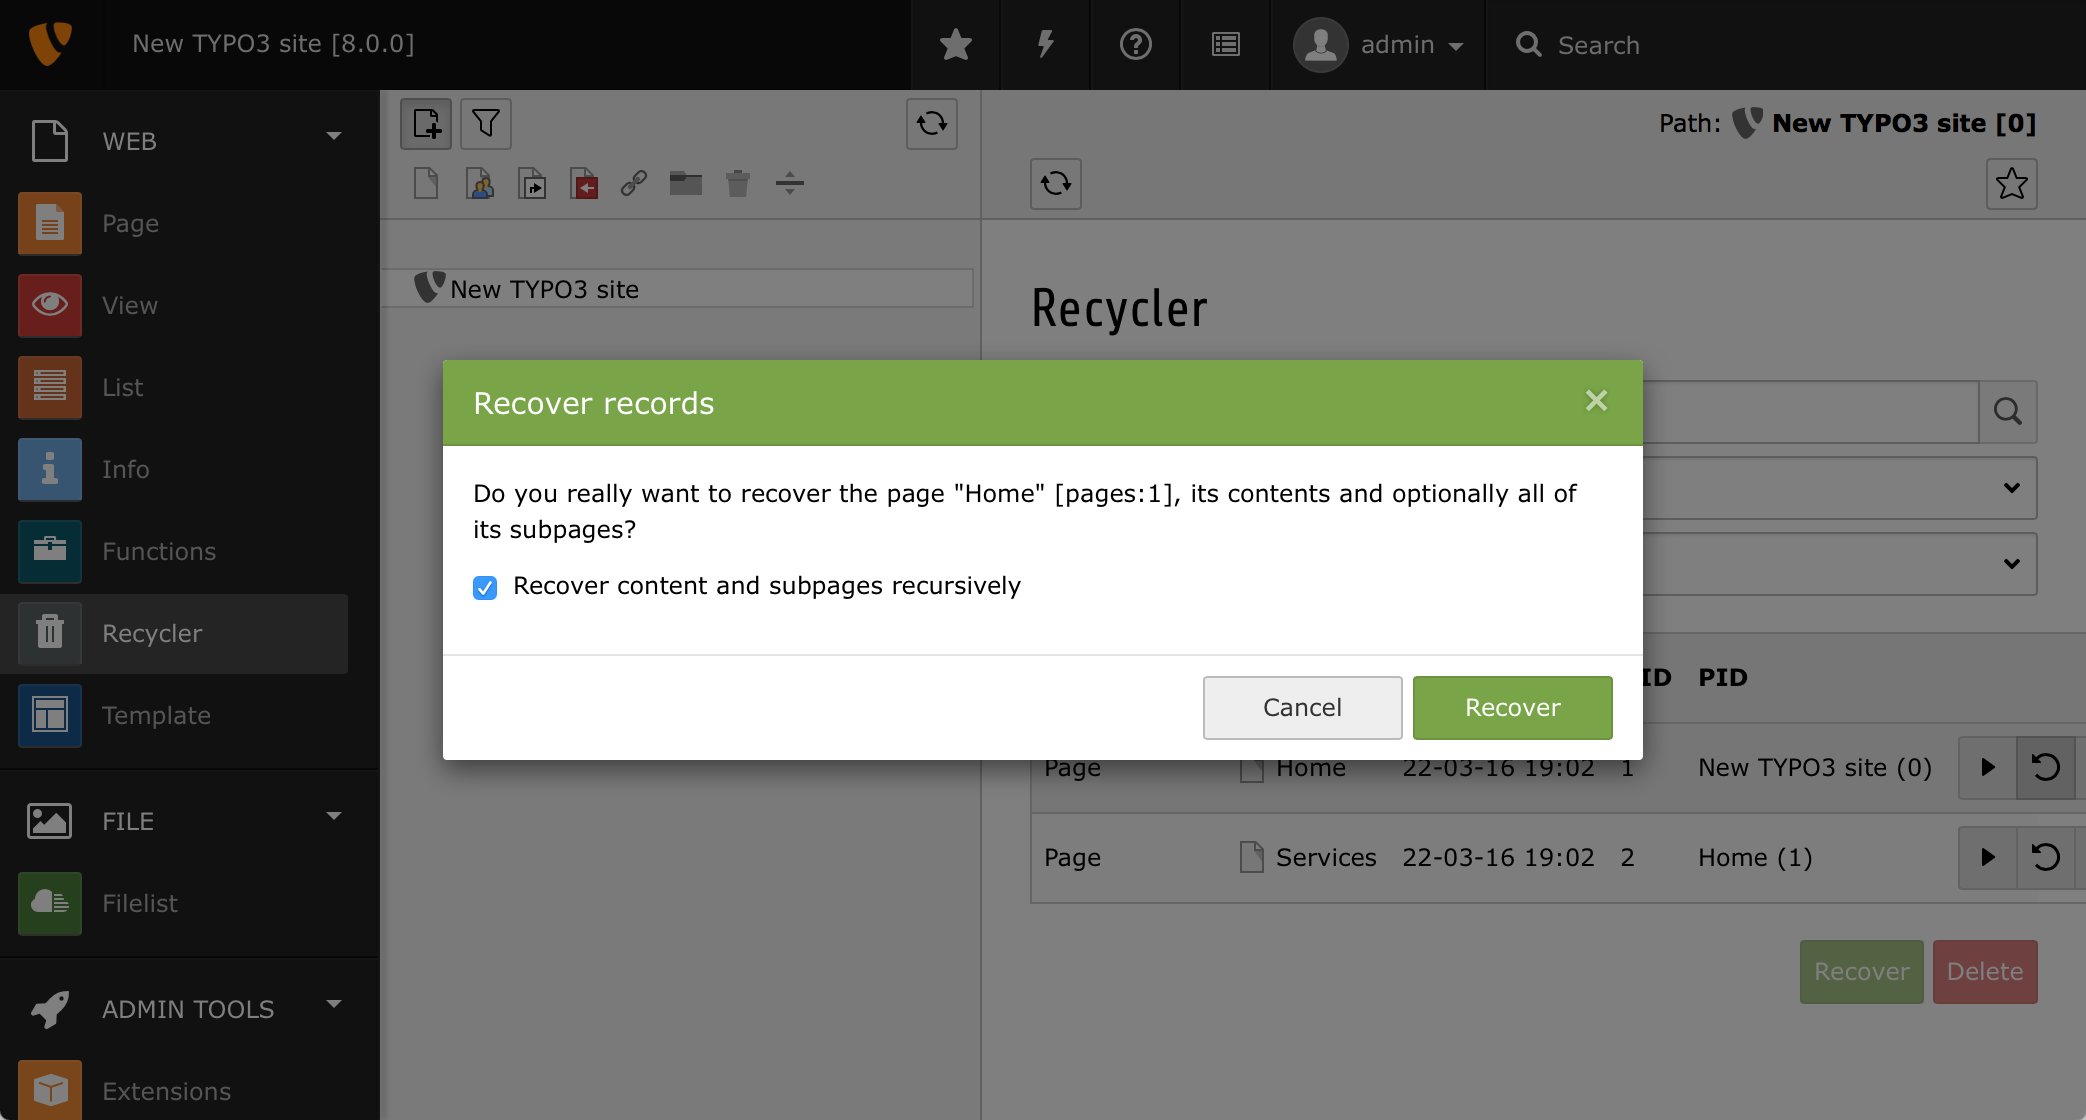
\includegraphics[width=0.70\linewidth]{BackendUserInterface/1835.png}
	\end{figure}

\end{frame}

% ------------------------------------------------------------------------------
% LTXE-SLIDE-START
% LTXE-SLIDE-UID:		866ee326-998c866e-fd3f0375-d71ec0ae
% LTXE-SLIDE-ORIGIN:	04855567-dac16e24-f5274c64-f1d49c36 English
% LTXE-SLIDE-TITLE:		EXT:form - Directly load form wizard as inline wizard
% LTXE-SLIDE-REFERENCE:	!Feature-69394-EXTform-DirectlyLoadFormWizardAsInlineWizard.rst
% ------------------------------------------------------------------------------
\begin{frame}[fragile]
	\frametitle{Interfaz de Usuario de Backend}
	\framesubtitle{Cargue directamente el asistente del formulario como asistente inline}

	El asistente de EXT:form es cargado directamente como asistente inline.
	No es necesario ya guardar y recargar el elemento de contenido recién creado para ser capaces de abrir el asistente. Esto es una gran mejora de usabilidad.

	\begin{figure}
		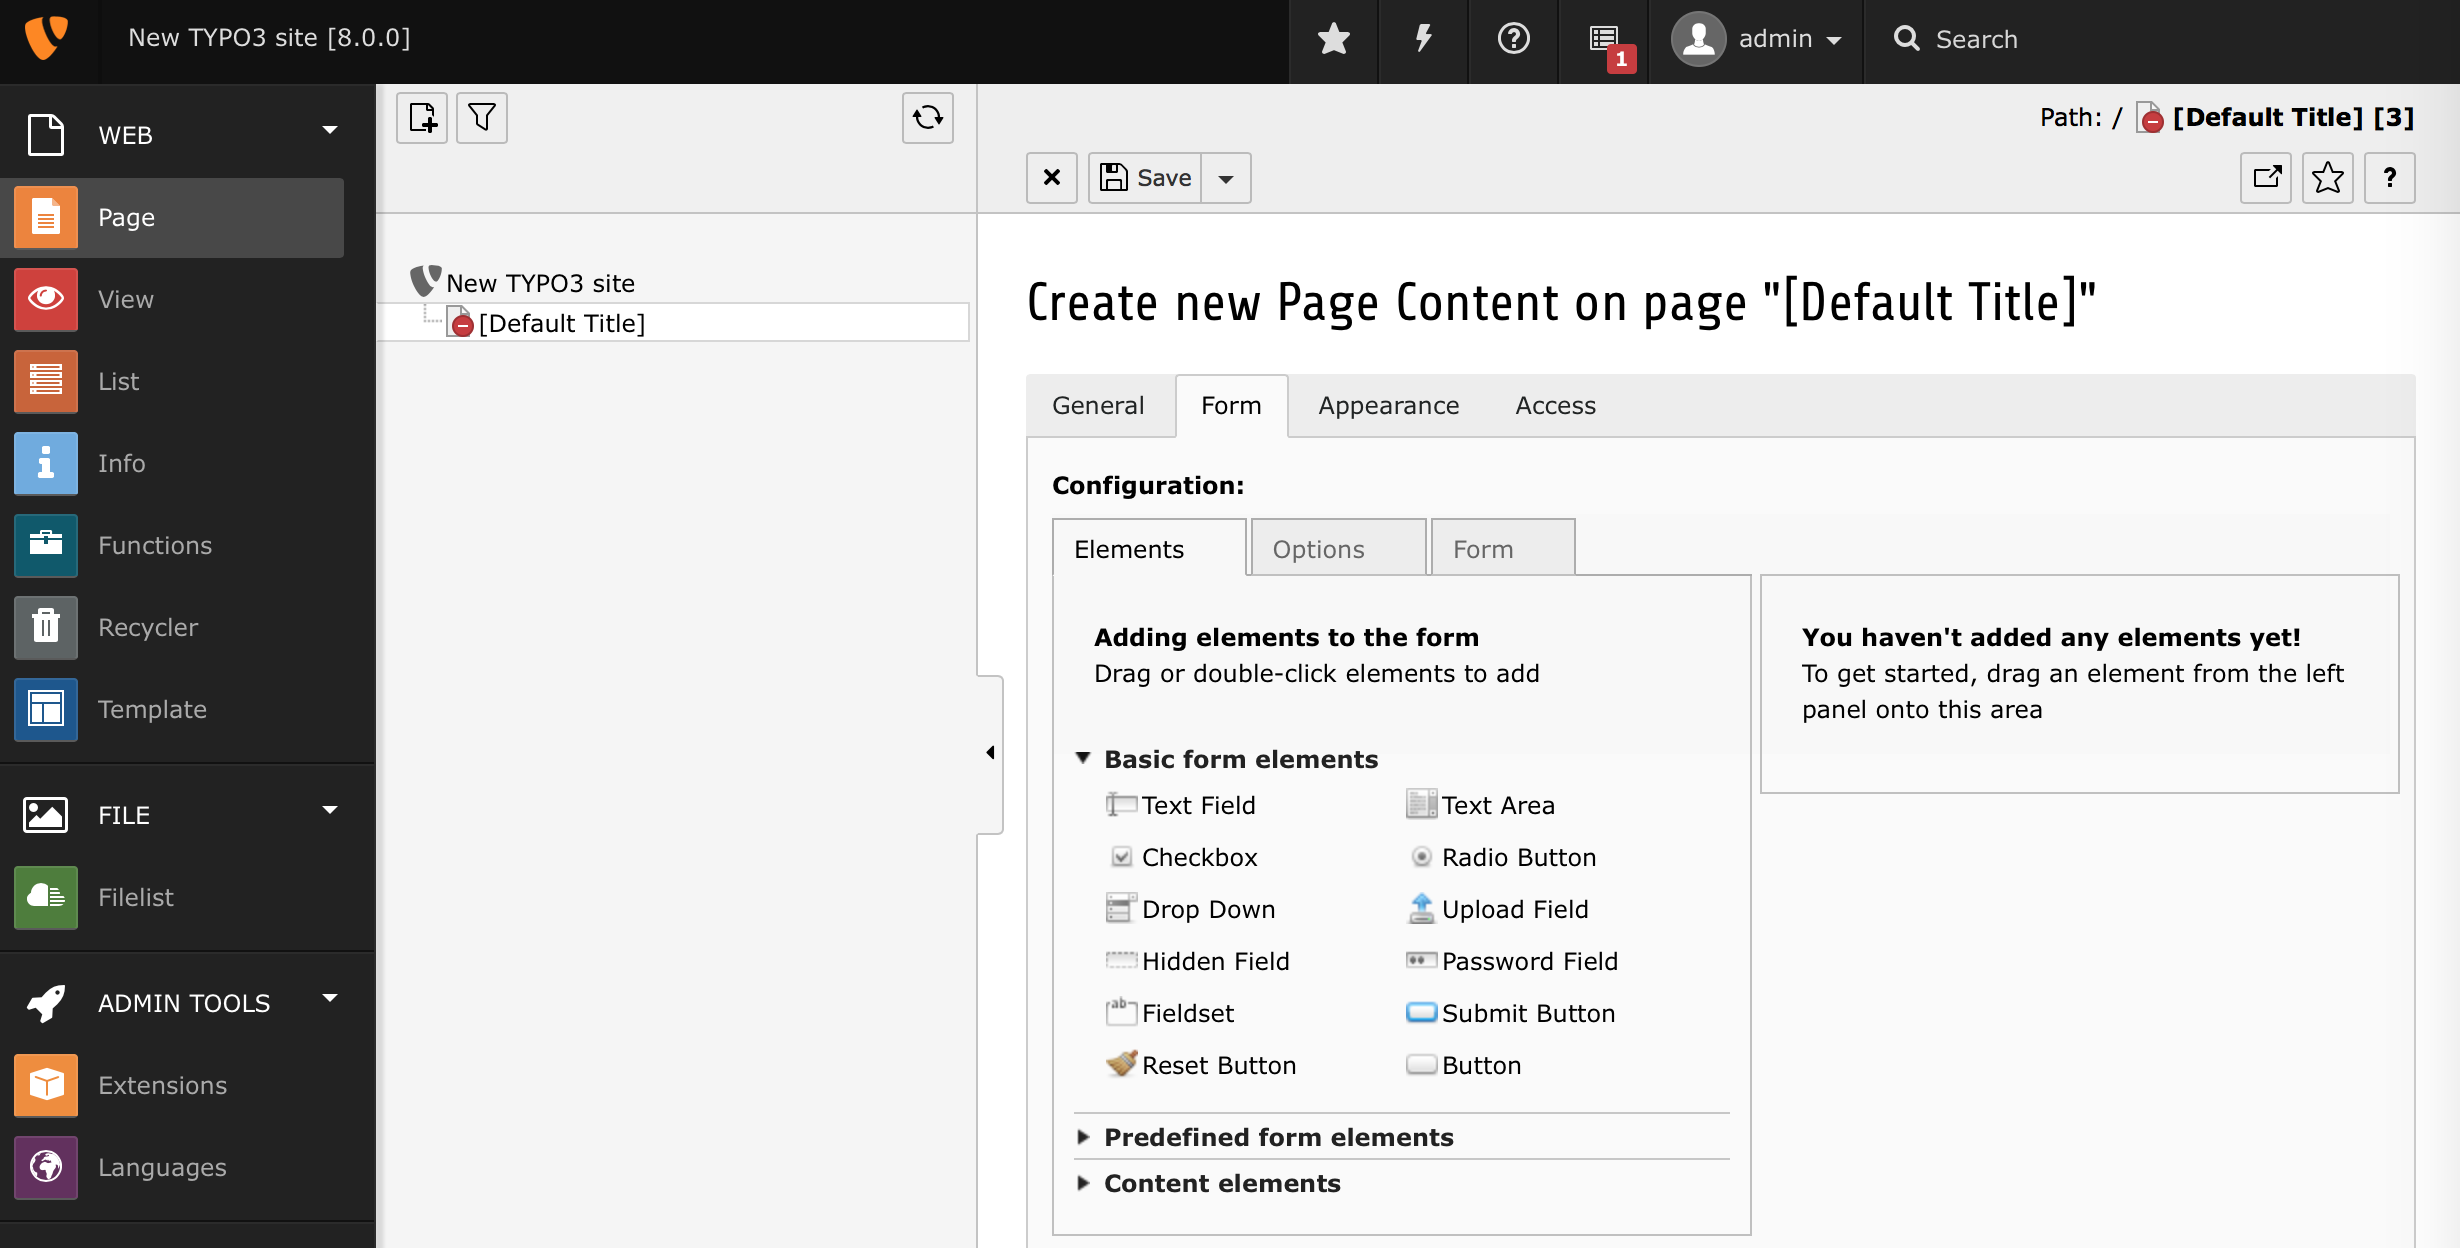
\includegraphics[width=0.70\linewidth]{BackendUserInterface/69394.png}
	\end{figure}

\end{frame}

% ------------------------------------------------------------------------------
% LTXE-SLIDE-START
% LTXE-SLIDE-UID:		15000145-31be5689-53b496b2-345f5af4
% LTXE-SLIDE-ORIGIN:	fd6d762a-b268caf0-cb6f9195-f553e035 English
% LTXE-SLIDE-TITLE:		Set the alternative backend logo via Extension Manager
% LTXE-SLIDE-REFERENCE:	!Feature-74109-SetTheAlternativeBackendLogoViaExtensionManager.rst
% ------------------------------------------------------------------------------
\begin{frame}[fragile]
	\frametitle{Interfaz de Usuario de Backend}
	\framesubtitle{Configure un logo alternativo para el backend vía Manejador de Extensiones (1)}

	El logo del backend en la esquina superior izquierda puede ahora configurarse en la configuración de la extensión
	EXT:backend en el Manejador de Extensiones.\newline
	Las opciones de configuración son:

	\begin{itemize}
		\item recurso como una ruta relativa de la instalación de TYPO3\newline
			\smaller
				p.e. "\texttt{fileadmin/images/my-background.jpg}"
			\normalsize

		\item ruta a una extensión\newline
			\smaller
				p.e. "\texttt{EXT:my\_theme/Resources/Public/Images/my-background.jpg}"
			\normalsize
	\end{itemize}

\end{frame}

% ------------------------------------------------------------------------------
% LTXE-SLIDE-START
% LTXE-SLIDE-UID:		15000145-31be5689-53b496b2-345f5af4
% LTXE-SLIDE-ORIGIN:	fd6d762a-b268caf0-cb6f9195-f553e035 English
% LTXE-SLIDE-TITLE:		Set the alternative backend logo via Extension Manager
% LTXE-SLIDE-REFERENCE:	!Feature-74109-SetTheAlternativeBackendLogoViaExtensionManager.rst
% ------------------------------------------------------------------------------
\begin{frame}[fragile]
	\frametitle{Interfaz de Usuario de Backend}
	\framesubtitle{Configure un logo alternativo para el backend vía Manejador de Extensiones (2)}

	\begin{itemize}
		\item un recurso externo\newline
			\smaller
				p.e. "\texttt{//example.com/my-background.png}"
			\normalsize

	\end{itemize}

	\begin{figure}
		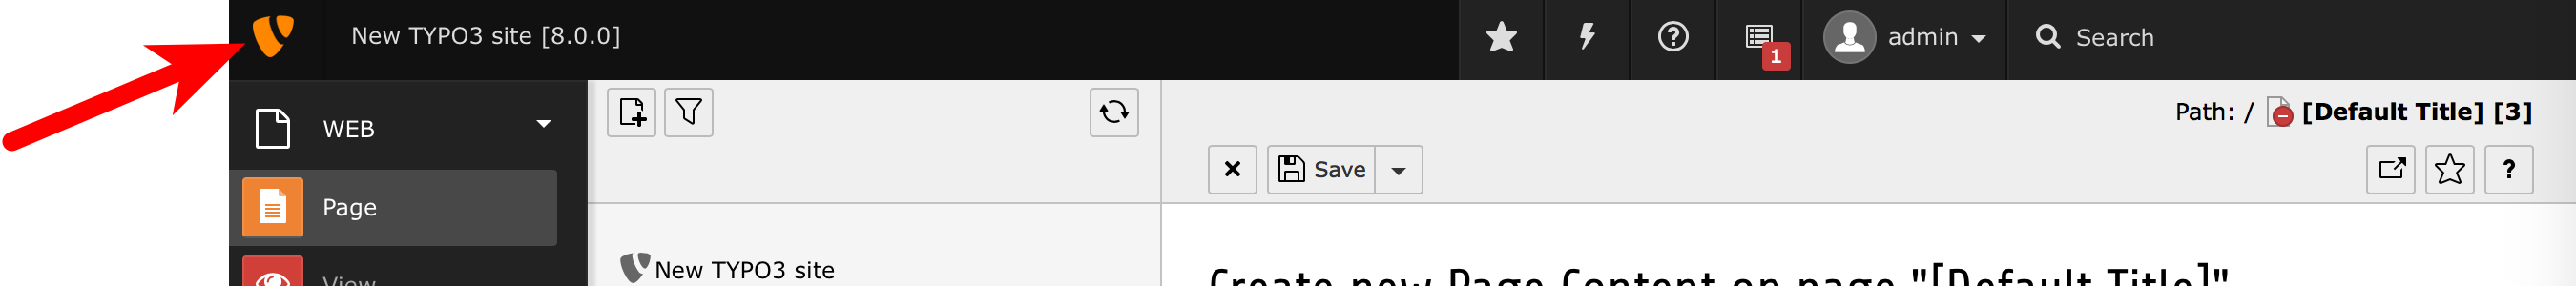
\includegraphics[width=0.7\linewidth]{BackendUserInterface/74109.png}
	\end{figure}

\end{frame}

% ------------------------------------------------------------------------------
% LTXE-SLIDE-START
% LTXE-SLIDE-UID:		5582a589-34b086cb-861788b6-69cc2745
% LTXE-SLIDE-ORIGIN:	ab5ef36b-c670fbea-fd6d762a-cb6f9195 English
% LTXE-SLIDE-TITLE:		Page module: drag and drop supports copying now
% LTXE-SLIDE-REFERENCE:	!Feature-74179-PageModuleDragDropCanDoCopiesViaCTRLKeyNow.rst
% ------------------------------------------------------------------------------
\begin{frame}[fragile]
	\frametitle{Interfaz de Usuario de Backend}
	\framesubtitle{Copie páginas en modo arrastrar \& soltar}

	Además de la característica usual de arrastrar y soltar en el módulo de página (que \textit{movía} elementos de contenido),
	ahora es posible crear copias: pulse la tecla CTRL mientras arrastra para crear una copia del elemento
	arrastrado. Después de que el arrastre se ha completado, el módulo de página se recargará para asegurar que el nuevo elemento será
	generado con toda la información necesaria.

	\begin{figure}
		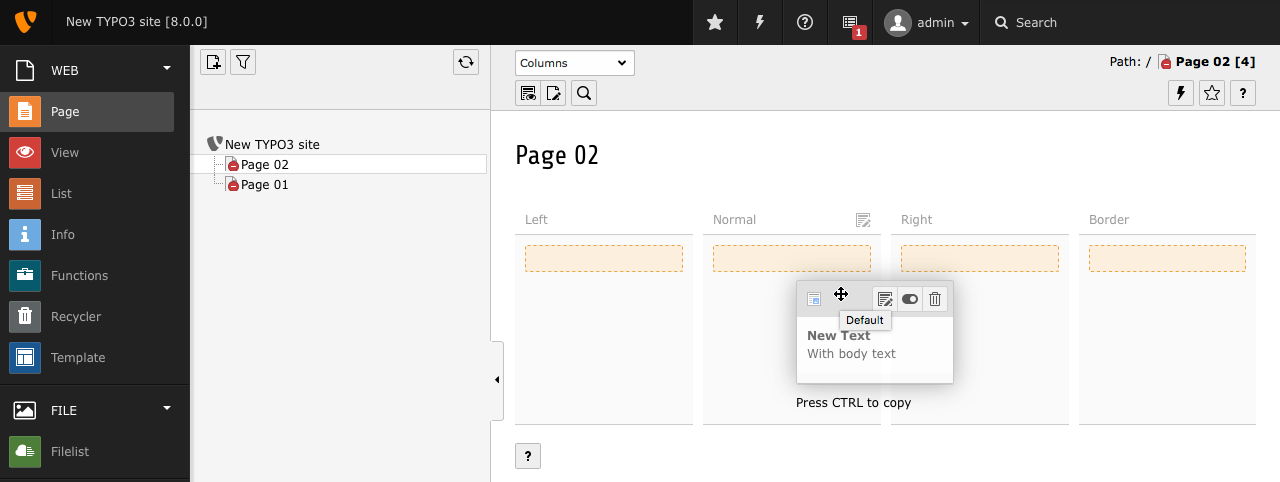
\includegraphics[width=0.7\linewidth]{BackendUserInterface/74179.png}
	\end{figure}

\end{frame}

% ------------------------------------------------------------------------------
